\documentclass{article}

% Más opciones para enumerar
\usepackage{enumitem}

% Formato de página
\usepackage[letterpaper, margin = 1.5cm]{geometry}

% Manejo de imágenes
\usepackage{graphicx}
\usepackage{wrapfig}
\graphicspath{{img/}}

\begin{document}
    \title{
        Fundamentos de bases de datos \\
        Tarea 2 \\
        Modelo Entidad/Relación
    }
    \author{
        Díaz Gómez Silvia \\
        Eugenio Aceves Narciso Isaac \\
        Quiroz Castañeda Edgar
    }
    \date {
        4 de marzo del 2019    
    }
    \maketitle

    \section{Repaso de conceptos generales}

    \begin{enumerate}[label = (\alph*)]
        % a
        \item {
            Un conjunto de \textbf{entidades débiles} siempre se puede convertir
            en un conjunto de \textbf{entidades fuertes} añadiendole a sus 
            atributos la \textbf{llave primaria} de conjunto de entidades fuertes
            a la que está asociado. Describe qué tipo de redundancia resultaría 
            si se realiza dicha conversión. \\
            Esto haría que las instancias de la entidad débil estén sujetas a 
            una única instancia de la entidad fuerte, pues las llaves son únicas. 
            Entonces, si antes de agregar la llave, una instancia débil $D$ 
            pertenece a varias instancias fuertes $F_0, ..., F_n$, al momento 
            de agregar la llave, $D$ ya no sería una instancia válida, pues su
            llave estaría multivaluada. Entonces, habría que crear nuevas 
            instancias $D_0, ..., D_n$ donde $D_i$ tendría la llave de $F_i$,
            pero en todos sus demás atributos, todas las $D_i$ tendrían 
            exactamente la misma información. Por lo que toda esa información 
            repetida sería reduntante.
        }
        % b
        \item {
            Responde a las siguientes cuestiones, deberás indicar 
            \textbf{si son posibles o no}, justificando tu respuesta. Cuando no 
            sea posible deberás indicar alguna recomendación al respecto.
            \begin{itemize}
                \item ¿Un \textbf{atributo compuesto} puede ser \textbf{llave}? \\
                    Sí puede serlo. Sólo hay que seguir garantizando que sea 
                    una combinación única e inmutable de atributos.
                \item ¿Un \textbf{atributo multivaluado} puede ser \textbf{llave}? \\
                    No puede serlo. Al ser varios, tenerlos como llave implicaría
                    tener varias llaves para la misma instancia, lo cuál no está
                    permitido.
                \item ¿Un \textbf{atributo derivado} puede ser llave? \\
                    Sí, siempre y cuando el proceso que se utilice para calcularlo
                    sea una función invertible que sólo dependa de atributos que 
                    nunca cambien. De cualquier manera, en caso de que se 
                    requiera usar un atributo derivado como llave, sería más 
                    eficiente usar como llave (tal vez compuesta) los atributos
                    que se usaron para calcularla.
                \item ¿Un \textbf{atributo multivaluado} puede ser 
                \textbf{compuesto}? \\
                    Sí puede serlo. Y sus componentes también serán multivaluedas.
                \item ¿Un \textbf{atributo multivaluado} puede ser \textbf{derivado}?
                    Sí puede serlo. Los atributos de los que se calcula deberían
                    ser o multivaluados o en algún paso del proceso se debe 
                    utilizar un parámetro multivaluado.
                \item ¿Qué implicaría la existencia de una \textbf{entidad} cuyos
                atributos sean \textbf{todos derivados}? \\
                    Que no va a tener atributos almacenados, por lo que durante la 
                    traducción al MR su ``tabla'' estaría vacía, por lo que no sería
                    una tabla. Es decir, al hacer la traducción ya no sería una 
                    entidad.
            \end{itemize} 
        }
        % c
        \item {
            Explica el concepto de \textbf{agregación} en el \textbf{modelo E/R}
            y proporciona un par de ejemplos.    
        }
        % d
        \item {
            Diseña un \textbf{modelo E/R} en donde reflejes los conceptos 
            revisados para el tema de \textbf{Modelo E/R} (no consideres el 
            \textit{Modelo E/R extendido}).
        }
    \end{enumerate}

    \section{Modelo Entidad/Relación}
    \begin{enumerate}[label = (\alph*)]
        \item {
            \textbf{Instalaciones deportivas} \\
            Un \textbf{centro de instalaciones deportivas} quiere hacer una
            aplicación para reservar serivicios de sus clientes. En el centro
            existen \textbf{instalaciones deportivas} (piscinas, gimnasios, 
            frontones, etc.). El centro tiene socios, de los cuales se 
            almacenan: CURP, nombre completo, dirección, teléfono de contacto,
            corroe electrónico, estado y la edad. A cada socio de le entrega 
            una \textbf{credencial de acceso} que tiene un número de socio, 
            fecha de expedición, vigencia. El centro cuenta con una serio de 
            \textbf{artículos} que se pueden rentar en un conjunto con la 
            reservación (balones, redes, raquetes, etc.). \\
            Cada instalación es reservada por un socio en una 
            \textbf{fecha determinada} y cuenta con una \textbf{hora de inicio}
            y una \textbf{hora de finalización}, siempre y cuando esté al 
            día con el pago de sus cuotas. Cada reservación puede tener 
            asociada uno o varios artículos deportivos que se alquilan aparte.
            Por ejemplo, si deseamos realizar una reservación para jugar 
            voleibol, se debe reservar una instalación con una cancha
            pertinente, una red y un balón. \\
            El diagrama propuesto es 
            \begin{center}
                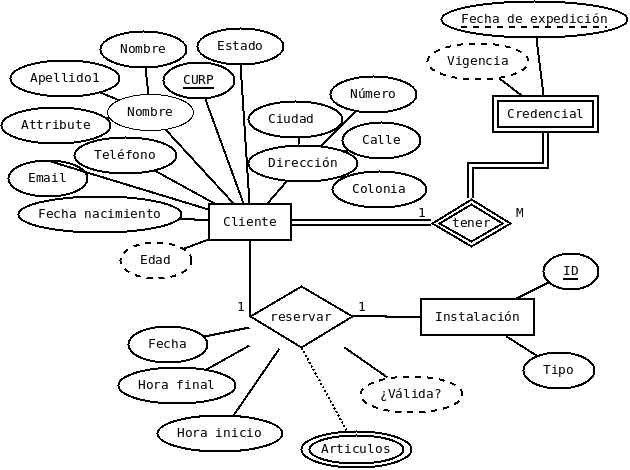
\includegraphics[width=0.75\textwidth]{deportes-er.png}
            \end{center}  
 
        }
        \item {
            \textbf{Sistema de información geográfica} \\
            La \textbf{Secretaría de Medio Ambiente y Recursos naturales 
            (SEMARNAT)} desea crear un \textbf{SIG} (Sistema de información
            Geográfica) para acceso público a través de Internet. El sistema 
            ofrecerá la siguiente información :
            \begin{itemize}
                \item {
                    Datos referentes a \textbf{ríos, afluentes, sistemas 
                    montañosos, montañas y municipios} donde se localizan.
                }
                \item {
                    De los \textbf{ríos} se alamcenará un identificador del
                    río, nombre, descripció y longitud total. Para cada río,
                    además, se almacenarán los municipios que atraviesa la 
                    longitud del tramo del río para cada municipio bañado.
                }
                \item {
                    De los \textbf{municipios} se almacenará un identificador
                    para el municipio, nombre y número de habitantes.
                }
                \item {
                    Los \textbf{ríos} pueden ser afluentes de otros ríos. Si
                    es el caso, se desea conocer a cuál río alimentan y el 
                    municipio en el que se unen al río del que son afluyentes.
                }
                \item {
                    En cuanto a los \textbf{sistemas montañosos}, se 
                    almacenará un código, el nombre, l orientación (norte, 
                    sur, este, oeste), la longitud, la altura mima y los 
                    municipios que ocupa. Los sistemas están formados por 
                    \textbf{montañas} de los que se almacena un código, un 
                    nombre, descripción y altura. Se debe considerar que una 
                    montaña sólo pertenecerá a un sistema motañoso. Se 
                    requiere también almacenar el municipio o municipios en
                    los que se encuentra, ya que hay casos en los que una 
                    montaña es compartida por varios municipios.
                }
                \item {
                    Las \textbf{montañas} además pueden tener un 
                    \textbf{origen volcánico} o de \textbf{plegamiento}. En
                    el caso de que su origen sea volcánico, se desea 
                    almacenar el tipo de volcán y si es plegamiento, se 
                    almacenará el periodo geológico de dicho plegamiento.
                }
                \item {
                    \textbf{Algunos ríos} y \textbf{montañas} son elementos 
                    geológicos \textbf{monitoreados por satélite}. De dichos 
                    elementos se desea almacenar la fecha en la que se 
                    comienzan a monitorear y el satélite que realiza el 
                    seguimiento. Un satélite puede minotoreae varios 
                    elementos. De satélites se desea almacenar su 
                    identificador, nombre y descripción.
                }
            \end{itemize}
        }
        \item {
            \textbf{Estrella de la muerte} \\
            Hace mucho tiempo, en una Galaxia muy, muy lejana, el malvado 
            \textbf{Imperio Galáctico} comenzó la construcción de su última arma
            , la \textbf{Estrella de la Muerte}, una estación espacial blindada
            con suficiente poder para destruir un plantea entero. Este terror 
            tecnoógico almacenará toda su información en una \textbf{base de 
            datos relacional}, y se te ha pedid diseñar un esquema E/R. La 
            solicitud que ha hecho el \textbf{Emperador} es la siguiente.
            \begin{itemize}
                \item {
                    La \textbf{Estrella de la Muerte} emplea una fuerza de 
                    trabajo de más de 200,000 trabajadores. Cada trabajador 
                    tiene asignado un \textbf{número de identificación Imperial}
                    , un \textbf{nombre} y \textbf{rango}. Los trabajadores 
                    pueden ser \textbf{oficiales, soldados de asalto, pilotos, 
                    artilleros} o \textbf{personal de apoyo} de la estación. 
                    Todo personal de la estación tiene un \textbf{oficial} al 
                    mando.
                }
                \item {
                    La estación se divide en varios niveles, cada uno 
                    identificado por un \textbf{número}. La base debe realizar
                    un seguimiento de la \textbf{superficie total} de un nivel,
                    la \textbf{capacidad de almacenamiento}, y si se trata de un 
                    \textbf{nivel restringido o no}. Todos los niveles tienen 
                    \textbf{viviendas} con capacidad de alojar a varios 
                    trabajadores, y a todos los trabajadores se les asignan 
                    viviendas de la estación.
                }
                \item {
                    Los trabajadores \textbf{pueden moverse} a través de otros 
                    niveles en la estación, siempre y cuando se les haya 
                    \textbf{brindado acceso} a esos niveles. La base de datos 
                    debe registrar la información de los \textbf{niveles} a los 
                    que cada \textbf{trabajador está autorizado} a acceder. Es 
                    importante destacar que algunos niveles no pueden tener 
                    ningún trabajador autorizado.
                }
                \item {
                    Algunos de los niveles de la estación pueden tener 
                    \textbf{bloques de celdas} para prisioneros y estos bloques
                    de celdas se identifican por una \textbf{sola letra} que es 
                    única dentro de un nivel; sin embargo estas letras se pueden
                    repetir entre los niveles. Cada celda tiene una cierta 
                    \textbf{capacidad de prisioneros} (\textit{no es la misma 
                    para todoas}). Para los \textbf{bloques de celdas} se deben
                    llevar un registro de la fecha de entrada y la fecha de 
                    ejecución del prisionero. Los prisioneros tiene un 
                    \textbf{identificador único}, un \textbf{nombre}, y una 
                    \textbf{afiliación} (por ejemplo, la escoria Rebelde).
                }
                \item {
                    Algunos de los niveles de la estación funcionan como 
                    \textbf{hangares}, donde se tienen \textbf{cruceros 
                    imperiales, naves de reconocimiento} y de \textbf{ataque}.
                    Cada nave tiene un \textbf{identificador único, capacidad de
                    vuelo, personal asignado} (\textit{oficiales, pilotos, 
                    personal de aopyo, soldados, etc.}), \textbf{armamento} y 
                    \textbf{hangar} al que está adignada.
                }
            \end{itemize}
        }
    \end{enumerate}

    \section{Ingeniería inversa}

    \begin{wrapfigure}{r}{0.40\textwidth}
        \centering
        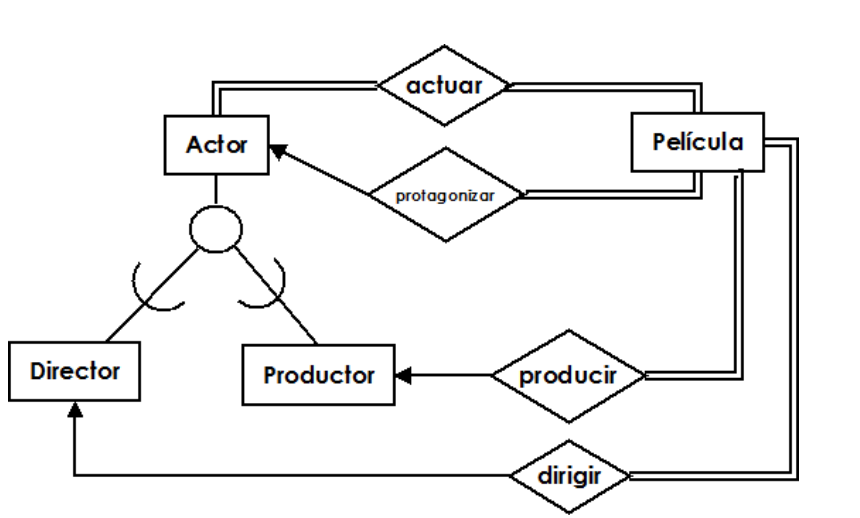
\includegraphics[width=0.40\textwidth]{peliculas-er.png}
    \end{wrapfigure}

    Considera el esquema \textbf{E/R} para la base de datos \textbf{Películas} 
    de la figura siguiente y asume que la base de datos está poblada. 
    \textbf{Actor} se utiliza como término genérico e incluye actrices. Dadas 
    las restricciones mostradas en el esquema \textbf{E/R}, responde a las 
    siguientes afirmaciones con \textbf{Verdadero, Falso} o \textbf{Quizás}
    (\textit{asigna está última respuesta a las afirmaciones que, no pudiendo 
    mostrarse como Verdaderas, tampoco se puede mostrar que son Falsas basandose
    en el esquema mostrado}).

    \textbf{Justifica TODAS tus respuestas}

    \begin{itemize}
        \item {
            En esta base de datos no hay ningún actor que no haya actuado en 
        ninguna película
        }
        \item {
            Hay algunos actores que han actuado en más de diez películas.
        }
        \item {
            Algunos actores han sido protagonistas en varias películas.
        }
        \item {
            Una película sólo puede tener un máximo de dos protagonistas.
        }
        \item {
            Cada director ha sido actor en alguna película.
        }
        \item {
            Ningún productos ha sido actor alguna vez.
        }
        \item {
            Un productor no puede ser actor en alguna otra película.
        }
        \item {
            Hay películas con más de una docena de actores.
        }
        \item {
            Algunos productores también han sido directores.
        }
        \item {
            La mayoría de las películas tienen un director y un productor.
        }
        \item {
            Algunas películas tienen director, pero varios productores.
        }
        \item {
            Hay algunos actores que han interpretado el papel de protagonista, 
            dirigido una película y producido alguna otra.
        }
        \item {
            Ninguna película tiene un director que también haya actuado en ella.
        }
        
    \end{itemize}

\end{document}